\documentclass[11pt]{article}
\usepackage[cm]{fullpage}
\usepackage{amsmath}
\usepackage{graphicx}

\begin{document}

\paragraph{Newton-Raphson step.}
Quadratic expansion
\[
    E
    \approx
    E_0
    +
    \Delta\mathbf{x}^\mathrm{t}
    \mathbf{g}_0
    +
    \tfrac{1}{2}
    \Delta\mathbf{x}^\mathrm{t}
    \mathbf{H}_0
    \Delta\mathbf{x}
    \qquad
    \Delta\mathbf{x}
    \equiv
    \mathbf{x}
    -
    \mathbf{x}_0
\]
Linear gradient expansion
\[
    \mathbf{g}
    =
    \mathbf{g}_0
    +
    \mathbf{H}
    \Delta\mathbf{x}
\]
Setting the gradient at the next point to zero gives the Newton-Raphson step
\[
    \mathbf{g}
    \overset{!}{=}
    \mathbf{0}
    \implies
    \Delta\mathbf{x}
    =
    -
    \mathbf{H}_0^{-1}
    \mathbf{g}_0
\]
For a perfectly quadratic surface, the Hessian is constant and the
Newton-Raphson step takes us directly to the stationary point.
On a surface with cubic and higher-order terms, this step can be repeated
iteratively until we are close enough to the stationary point that the region
separating us from it is approximately quadratic.


\paragraph{The secant condition.}
For points
\(
    \mathbf{x}
\)
and
\(
    \mathbf{x}_0
\)
sharing a locally quadratic region with each other, the change in the gradient
between them is described by the following.
\[
    \mathbf{H}
    \Delta\mathbf{x}
    \approx
    \mathbf{H}_0
    \Delta\mathbf{x}
    \approx
    \Delta\mathbf{g}
    \qquad
    \Delta\mathbf{g}
    \equiv
    \mathbf{g} - \mathbf{g}_0
\]
This can be used to determine an approximation
\(
    \tilde{\mathbf{H}}
\)
to the Hessian at
\(
    \mathbf{x}
\)
using the Hessian at
\(
    \mathbf{x}_0
\).
Namely, we require the approximation to satisfy
\[
    \tilde{\mathbf{H}}
    \Delta\mathbf{x}
    \overset{!}{=}
    \Delta\mathbf{g}
    \qquad
    \tilde{\mathbf{H}}
    =
    \mathbf{H}_0
    +
    \Delta\tilde{\mathbf{H}}
\]
which is known as the {\itshape quasi-Newton condition}, or alternatively the
{\itshape secant condition}.
If the dimension is \(d\), then we have \(d\) linear equations and \(d^2\)
undetermined matrix elements (or rather \(d(d+1)/2\) matrix elements, by
symmetry), so the system is underdetermined -- we have an infinite number of
solutions.

The simplest way forward is to assume \(\Delta\tilde{\mathbf{H}}\) has rank 1,
which for a symmetric matrix implies that it has the form
\[
    \Delta\tilde{\mathbf{H}}
    =
    \eta\,
    \mathbf{e}
    \mathbf{e}^\mathrm{t}
\]
where \(\eta\) is a scalar and \(\mathbf{e}\) is a unit vector.
This is the {\itshape symmetric rank-1} (SR1) approximation.
Substituting this into the secant condition, we find
\[
    \mathbf{e}
    =
    \frac{%
        \Delta\mathbf{g}
        -
        \mathbf{H}_0
        \Delta\mathbf{x}
    }{%
        \|
        \Delta\mathbf{g}
        -
        \mathbf{H}_0
        \Delta\mathbf{x}
        \|
    }
    \qquad
    \eta
    =
    \frac{%
        \mathbf{e}\cdot
        (
            \Delta\mathbf{g}
            -
            \mathbf{H}_0
            \Delta\mathbf{x}
        )
    }{%
        \mathbf{e}\cdot
        \Delta\mathbf{x}
    }
    =
    \frac{%
        (
            \Delta\mathbf{g}
            -
            \mathbf{H}_0
            \Delta\mathbf{x}
        )^2
    }{%
        (
            \Delta\mathbf{g}
            -
            \mathbf{H}_0
            \Delta\mathbf{x}
        )\cdot
        \Delta\mathbf{x}
    }
\]
which allows us to simplify the SR1 matrix update.
\[
    \Delta\tilde{\mathbf{H}}_{\mathrm{SR1}}
    \equiv
    \frac{%
        (
            \Delta\mathbf{g}
            -
            \mathbf{H}_0
            \Delta\mathbf{x}
        )
        (
            \Delta\mathbf{g}
            -
            \mathbf{H}_0
            \Delta\mathbf{x}
        )^\mathrm{t}
    }{%
        (
            \Delta\mathbf{g}
            -
            \mathbf{H}_0
            \Delta\mathbf{x}
        )\cdot
        \Delta\mathbf{x}
    }
\]
This provides a scheme for updating the Hessian using the change in the first
derivative as we move across the potential surface.
If we take several steps in a small, locally quadratic region of the surface,
this approximation will improve with each step, and eventually we will have
quite a good approximation to \(\mathbf{H}\).
We can determine other approximations by assuming that the Hessian correction
has rank 2, which can be used to derive the {\itshape
Broyden-Fletcher-Goldfarb-Shanno} (BFGS) and {\itshape Davidon-Fletcher-Powell}
(DFP) Hessian updates.

Combining secant updating with Newton-Raphson optimization leads to the
{\itshape quasi-Newton optimization algorithms}, which have the following form.
\begin{enumerate}
    \item
        Evaluate the gradient \(\mathbf{g}_0\) at the starting point
        \(\mathbf{x}_0\) and either evaluate the Hessian or use an
        approximation.
        Setting
        \(
            \tilde{\mathbf{H}}_0
            =
            \tfrac{\|\mathbf{g}_0\|}{s_0}
            \mathbf{1}
        \)
        will yield a gradient descent of length \(s_0\) for the initial step.
    \item
        \label{item:loop-step}
        Take a Newton-Raphson step.
        \[
            \mathbf{x}
            =
            \mathbf{x}_0
            +
            \Delta\mathbf{x}
            \qquad
            \Delta\mathbf{x}
            =
            -
            \mathbf{H}_0^{-1}
            \mathbf{g}_0
        \]
    \item
        Evaluate the gradient \(\mathbf{g}\) at the new point.
        If \(\max(\mathbf{g})<\mathrm{tol}\), quit.
        We have converged.
    \item
        Otherwise, update the Hessian using a secant method like SR1.
        \[
            \tilde{\mathbf{H}}
            =
            \tilde{\mathbf{H}}_0
            +
            \Delta\tilde{\mathbf{H}}_\mathrm{SR1}
            \qquad
            \Delta\tilde{\mathbf{H}}_\mathrm{SR1}
            =
            \frac{%
                (
                    \Delta\mathbf{g}
                    -
                    \mathbf{H}_0
                    \Delta\mathbf{x}
                )
                (
                    \Delta\mathbf{g}
                    -
                    \mathbf{H}_0
                    \Delta\mathbf{x}
                )^\mathrm{t}
            }{%
                (
                    \Delta\mathbf{g}
                    -
                    \mathbf{H}_0
                    \Delta\mathbf{x}
                )\cdot
                \Delta\mathbf{x}
            }
        \]
    \item
        Set
        \(
            \mathbf{x}_0\leftarrow \mathbf{x},
            \mathbf{g}_0\leftarrow \mathbf{g},
        \)
        and
        \(
            \mathbf{H}_0\leftarrow \mathbf{H}
        \)
        and return to step~\ref{item:loop-step}.
\end{enumerate}


\section*{Rational function optimization}

\noindent
Goal: Step to a position on the reaction path in the uphill direction
\[
    f
    \approx
    f_0
    +
    \Delta\mathbf{x}^\mathrm{t}
    \mathbf{g}_0
    +
    \tfrac{1}{2}
    \Delta\mathbf{x}^\mathrm{t}
    \mathbf{H}_0
    \Delta\mathbf{x}
\]

\noindent
Look for extrema subject to the constraint of a fixed step size:
\[
    \|\Delta\mathbf{x}\|
    \overset{!}{=}
    s
\]
This constraint defines an (\(n-1\))-dimensional surface.

For the two-dimensional case, this defines a circle.
Within a locally quadratic (bowl- or saddle-shaped) region, this circle will
have a pair of global maxima and minima 
(barring the case of a circularly symmetric potential)
\begin{center}
    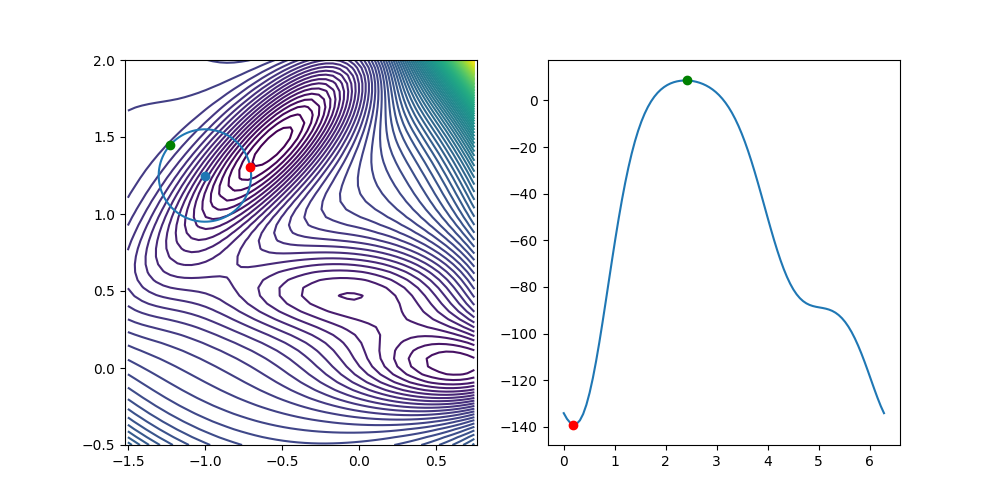
\includegraphics[width=0.8\linewidth]{figs/potential03.png}
\end{center}
and it may have up to one additional pair of local maxima and minima.
\begin{center}
    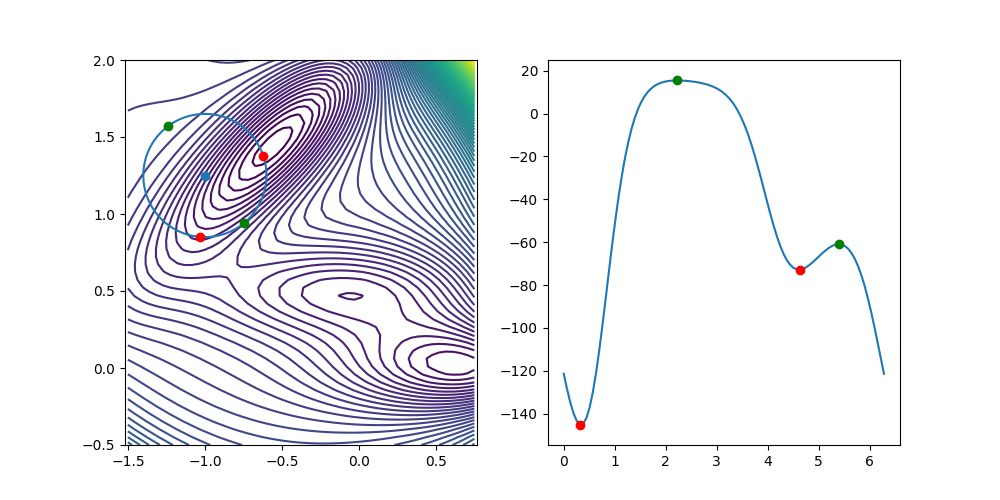
\includegraphics[width=0.8\linewidth]{figs/potential04.png}
\end{center}
Note that global minimum points downhill toward the bottom of the well, whereas
the local minimum points uphill toward the valley ridge.

\noindent
Lagrangian:
\[
    \mathcal{L}(\mathbf{x}, \lambda)
    =
    f_0
    +
    \Delta\mathbf{x}^\mathrm{t}
    \mathbf{g}_0
    +
    \tfrac{1}{2}
    \Delta\mathbf{x}^\mathrm{t}
    \mathbf{H}_0
    \Delta\mathbf{x}
    -
    \tfrac{\lambda}{2}
    (
        \Delta\mathbf{x}\cdot\Delta\mathbf{x}
        -
        s^2
    )
\]

\noindent
Setting the gradient of \(\mathbf{x}\) to zero gives a modified Newton-Raphson
step
\[
    \Delta\mathbf{x}
    \overset{!}{=}
    -
    (\mathbf{H}_0 - \lambda)^{-1}
    \mathbf{g}_0
\]

\noindent
Substituting this into the derivative of \(\lambda\) gives the following
\[
    s^2
    \overset{!}{=}
    \Delta\mathbf{x}\cdot\Delta\mathbf{x}
    =
    \mathrm{g}_0^\mathrm{t}
    (\mathbf{H}_0 - \lambda)^{-2}
    \mathrm{g}_0
\]
This algebraic equation determines the value of \(\lambda\) for a given value of
\(s\).
To understand it, expand it in the Hessian eigenbasis.
\[
    s^2
    =
    \sum_{i=1}^n
    \frac{g_{0,i}^2}{(h_{0,i} - \lambda)^2}
\]
\begin{enumerate}
    \item
        Right-hand side is positive for all \(\lambda\) and blows up to
        \(+\infty\) whenever \(\lambda\approx h_i\).
        Between the volcanoes we will have local minima.
    \item
        Thus, we can see that as we increase \(s^2\) we will have first
        \begin{enumerate}
            \item
                Two solutions at \(\lambda\rightarrow\pm\infty\) for
                \(s^2\rightarrow0\).
            \item
                Two solutions at \(\lambda<h_1\) and \(\lambda>h_n\) for small
                values of \(s^2\).
            \item
                Three solutions at \(\lambda<h_1\), \(h_k<\lambda<h_{k+1}\), and
                \(\lambda>h_n\) where we hit the first local minimum in \(s^2\).
            \item
                As \(s^2\) increases, the middle solution will split into two
                solutions between \(h_k<\lambda<h_{k+1}\) on either side of the
                well.
            \item
                Increasing numbers of solutions as we pass through other local
                minima.
        \end{enumerate}
\end{enumerate}


\end{document}
